\documentclass[]{article}
\usepackage{lmodern}
\usepackage{amssymb,amsmath}
\usepackage{ifxetex,ifluatex}
\usepackage{float}
\usepackage{fixltx2e} % provides \textsubscript
\usepackage{dcolumn}
\usepackage{multicol}
\usepackage{titling}
\usepackage[latin1]{inputenc}

% use upquote if available, for straight quotes in verbatim environments
\IfFileExists{upquote.sty}{\usepackage{upquote}}{}
% use microtype if available
\IfFileExists{microtype.sty}{%
\usepackage{microtype}
\UseMicrotypeSet[protrusion]{basicmath} % disable protrusion for tt fonts
}{}

\usepackage[margin=1in]{geometry}
\usepackage{hyperref}
\hypersetup{unicode=true,
            pdftitle={World's 50 Best Restaurants and Tourism},
            pdfauthor={Carrer L.},
            pdfborder={0 0 0},
            breaklinks=true}
\urlstyle{same}  % don't use monospace font for urls
\usepackage{color}
\usepackage{fancyvrb}
\newcommand{\VerbBar}{|}
\newcommand{\VERB}{\Verb[commandchars=\\\{\}]}
\DefineVerbatimEnvironment{Highlighting}{Verbatim}{commandchars=\\\{\}}

\usepackage{framed}
\usepackage{graphicx,grffile}
\makeatletter
\def\maxwidth{\ifdim\Gin@nat@width>\linewidth\linewidth\else\Gin@nat@width\fi}
\def\maxheight{\ifdim\Gin@nat@height>\textheight\textheight\else\Gin@nat@height\fi}
\makeatother
% Scale images if necessary, so that they will not overflow the page
% margins by default, and it is still possible to overwrite the defaults
% using explicit options in \includegraphics[width, height, ...]{}
\setkeys{Gin}{width=\maxwidth,height=\maxheight,keepaspectratio}
\IfFileExists{parskip.sty}{%
\usepackage{parskip}
}{% else
\setlength{\parindent}{0pt}
\setlength{\parskip}{6pt plus 2pt minus 1pt}
}
\setlength{\emergencystretch}{3em}  % prevent overfull lines
\providecommand{\tightlist}{%
  \setlength{\itemsep}{0pt}\setlength{\parskip}{0pt}}
\setcounter{secnumdepth}{0}


%%% Use protect on footnotes to avoid problems with footnotes in titles
\let\rmarkdownfootnote\footnote%
\def\footnote{\protect\rmarkdownfootnote}

% Create subtitle command for use in maketitle
\newcommand{\subtitle}[1]{
  \posttitle{
    \begin{center}\large#1\end{center}
    }
}
\setlength{\droptitle}{-2em}
\title{World's 50 Best Restaurants and Tourism}
\pretitle{\vspace{\droptitle}\centering\huge}
\posttitle{\par}
\author{Carrer L.}
\preauthor{\centering\large\emph}
\postauthor{\par}
\predate{\centering\large\emph}
\postdate{\par}
\date{10/10/2018}



\begin{document}
\maketitle



\subsection{Introduction}


Recently we have witnessing the growth of the so-called ``experience-based'' tourism as a result of the shift in consumer's value. Beside the common believe that food is one of the most important factor tourists take into account when it comes to travel destinations, there is also a wide literature confirming this belief. Although, food has always played been a critical factor in deciding the travel part of any holiday, the concept of traveling to a specific destination specifically for its restaurants scene is a recently new trend. 

Moreover, in recent years we are experiencing a growth of the number of TV Programs, magazines and books publicizing the industry of food as a whole, ranging from the so-called ``street-food'' to the high-end part of the business, which gather the gourmet restaurants and the niche of the ``Michelin-starred restaurants''. Therefore, such an exposure may have a positive effective in the decision-making of tourists.

The world's 50 best restaurant list produced by UK Media Company William Reed Business Media reflect the heterogeneity of the culinary landscape while giving a snapshot of ``heute cuisine''. In fact while the list is mostly comprised from restaurants based in go-to destinations, there are also restaurants in off-beaten paths such as the Faviken in north-western Sweden, more than 600 Kilometers north from Stockholm. The guest-to-be may wonder why the chef has chosen this location, while others may wonder why they guests would decide to take such a journey only to visit a restaurant. This is also the aim of hospitality management studies: why tourist pick a travel destination? Do they factor the presence of such important culinary destinations?

To shed some light on these questions the following analysis has been conducted: does the number of arrivals for international tourism obtained from the World Bank website have a correlation with the presence of the world's best 50 restaurants? 

A limitation of this work is that data on arrivals are gathered at country level, therefore further studies could actually benefit from the usage of local tourism data. Moreover, while this analysis focus only on the existence of a correlation between the above-mentioned set of data, it would be interesting to assess in further studies the direction of the casual relationship between having various restaurants in the top 50 ranking and the tourism. Indeed, it is not clear whether tourists are attracted to destinations where one can find a top restaurant or the other way around, that is, restaurants are established where the market size is bigger due to tourists inflow. 



\subsection{Data Scraping}

The data for the project on the 50 best restaurants was scraped directly from the website of the ``The World's 50 Best Restaurants", while the data on tourist arrivals was simply obtained from the website of The World Bank, International tourism, number of arrivals.

The data on the ranking is available only from 2003, while the data on tourism is available up until 2016. As such we delimit out analysis to the period 2003-2016.

Moreover, we only include in our analysis the countries for which at least one restaurant was included in the ranking at least one year.



\subsection{Results}




% Table created by stargazer v.5.2.2 by Marek Hlavac, Harvard University. E-mail: hlavac at fas.harvard.edu
% Date and time: Sun, Oct 14, 2018 - 16:44:10
% Requires LaTeX packages: dcolumn 
\begin{table}[!htbp] \centering 
  \caption{Correlation international tourist arrivals and number of restaurant} 
  \label{} 
\begin{tabular}{@{\extracolsep{5pt}}lD{.}{.}{-3} } 
\\[-1.8ex]\hline 
\hline \\[-1.8ex] 
 & \multicolumn{1}{c}{\textit{Dependent variable:}} \\ 
\cline{2-2} 
\\[-1.8ex] & \multicolumn{1}{c}{arrivals} \\ 
\hline \\[-1.8ex] 
 num\_restaurant & 183,388.400 \\ 
  & (125,618.500) \\ 
  & \\ 
 Constant & 1,033,445.000 \\ 
  & (962,115.200) \\ 
  & \\ 
\hline \\[-1.8ex] 
Year FE & \multicolumn{1}{c}{Yes} \\ 
Country FE & \multicolumn{1}{c}{Yes} \\ 
\hline \\[-1.8ex] 
Observations & \multicolumn{1}{c}{525} \\ 
R$^{2}$ & \multicolumn{1}{c}{0.977} \\ 
Adjusted R$^{2}$ & \multicolumn{1}{c}{0.975} \\ 
Residual Std. Error & \multicolumn{1}{c}{3,105,260.000 (df = 472)} \\ 
F Statistic & \multicolumn{1}{c}{391.177$^{***}$ (df = 52; 472)} \\ 
\hline 
\hline \\[-1.8ex] 
\textit{Note:}  & \multicolumn{1}{r}{$^{*}$p$<$0.1; $^{**}$p$<$0.05; $^{***}$p$<$0.01} \\ 
\end{tabular} 
\end{table} 



From the result on the table, we see that there is a positive impact on the number of restaurants present in the ranking and the number of arrivals in a given country. However, this coefficient is not statistically different from 0.

We could arrive to the same conclusion by looking at the graphs. The first is a scatter plot, depicting the averages over time of the number of arrivals and number of restaurants included in the ranking across countries.
The second one is a similar scatter plot, but instead of taking averages we plot the absolute numbers for each year.

\begin{figure}[H]
	\centering
	\textbf{Mean arrivals and number of restaurants across country}	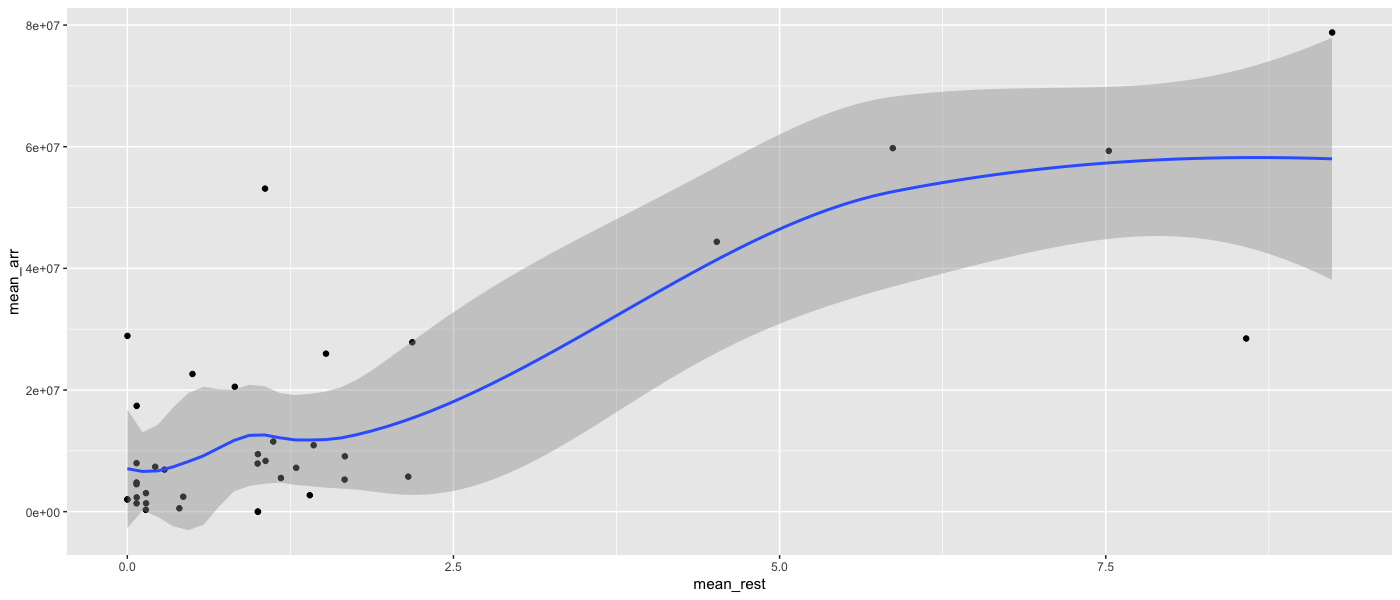
\includegraphics[width=0.9\textwidth]{../../output/graphs/graph_1.png}
\end{figure}

\begin{figure}[H]
	\centering
	\textbf{Arrivals and number of restaurants across country for each year}
	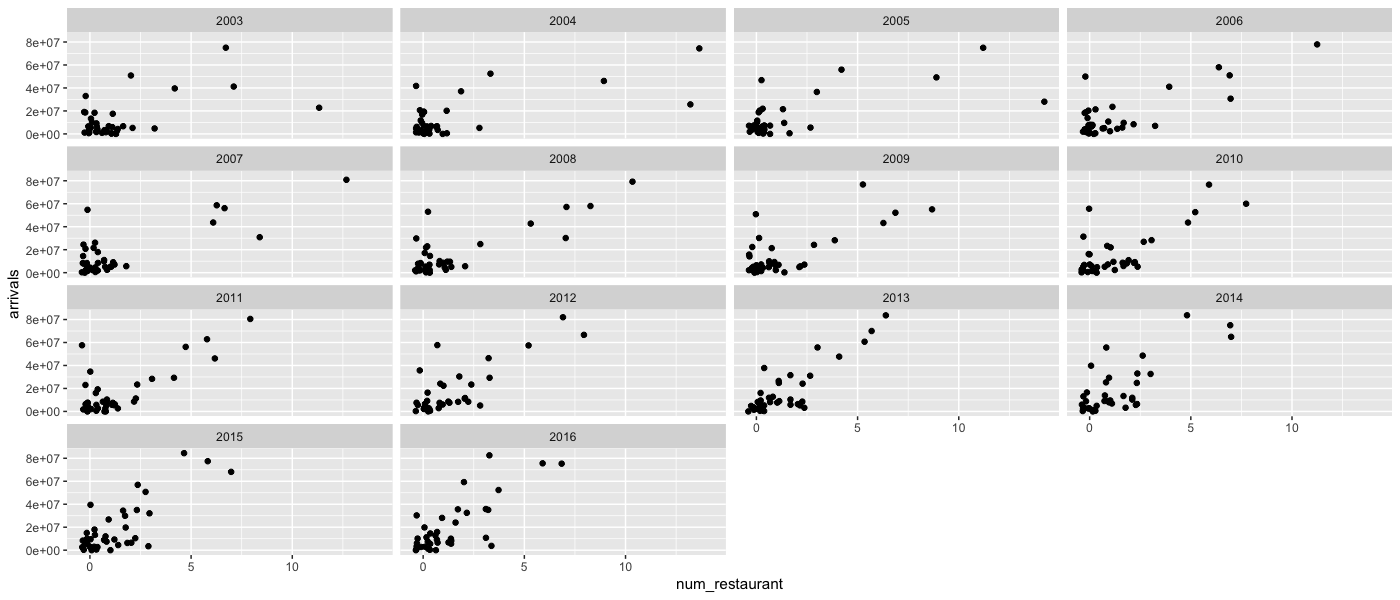
\includegraphics[width=0.9\textwidth]{../../output/graphs/graph_2.png}
\end{figure}



\subsection{Conclusion}

In this project, I have carried out a very simplistic investigation on the correlation between the number of intervational tourists arrivals in a given country and the numbers of restaurants which appear in the well-know list of the 50 best restaurants in the world. As previously mentioned, there is no causal analysis and I do not have data at the local level. An ideal follow-up study would try to establish this casual link in a rigourous manner by emplying local data.


\end{document}
